\documentclass[11pt]{article}
\usepackage[T1]{fontenc}
\usepackage[utf8]{inputenc}
\usepackage{lmodern,amsmath,amssymb,amsthm}
\usepackage[margin=1in]{geometry}
\usepackage{newunicodechar}
\usepackage{tikz}
\usetikzlibrary{arrows.meta}
\usepackage[title]{appendix}
\usepackage{hyperref}
\hypersetup{colorlinks=true,linkcolor=blue,citecolor=blue,urlcolor=blue,
  pdftitle={Counterexamples to the conjectured characterization of Hamiltonian degree sequences in digraphs},pdfauthor={P. Graham}}
\newtheorem{theorem}{Theorem}
\newtheorem{corollary}[theorem]{Corollary}
\newtheorem{lemma}[theorem]{Lemma}
\newtheorem{conjecture}{Conjecture}
\renewcommand{\theconjecture}{\Alph{conjecture}}
\newunicodechar{ℕ}{\ensuremath{\mathbb{N}}}
\newunicodechar{∀}{\ensuremath{\forall}}
\newunicodechar{∃}{\ensuremath{\exists}}
\newunicodechar{¬}{\ensuremath{\neg}}
\newunicodechar{∧}{\ensuremath{\wedge}}
\newunicodechar{∨}{\ensuremath{\vee}}
\newunicodechar{→}{\ensuremath{\to}}
\newunicodechar{≃}{\ensuremath{\simeq}}
\newunicodechar{≥}{\ensuremath{\geq}}
\newunicodechar{≤}{\ensuremath{\leq}}
\newunicodechar{⟨}{\ensuremath{\langle}}
\newunicodechar{⟩}{\ensuremath{\rangle}}
\title{Counterexamples to the conjectured characterization of Hamiltonian degree sequences in digraphs}
\author{P. Graham\\ \small\url{https://orcid.org/0009-0007-8493-1505}}
\date{November 4, 2026}
\begin{document}
\maketitle
\begin{abstract}
We show that the conjecture of Kühn, Osthus and Treglown (2008), which would characterize the degree sequences forcing a Hamilton cycle in a digraph, fails for every order $n\ge7$ and holds for $3\le n\le6$. It states that every digraph whose separately sorted out- and in-degree sequences satisfy two Chvátal-type conditions, and a third condition when the order is even, has a Hamilton cycle. It strengthens Nash-Williams' conjecture of 1975, which assumes strong connectivity instead of the third condition. Guninski found 6-vertex counterexamples to Nash-Williams' conjecture on MathOverflow in 2013 and 2020; the 2013 example was confirmed there by Royle and Thomas and the 2020 ones by DeBiasio. All of them violate the third condition. Our counterexamples are an explicit 7-vertex digraph and an explicit family, and the small orders are settled by exhaustive search. Hence Nash-Williams' conjecture fails for every $n\ge7$, in addition to Guninski's case $n=6$, and the same search shows that it holds for $3\le n\le5$. The family also shows that for every $n\ge8$ the conditions of either conjecture do not even force a cycle through every pair of vertices, answering a question recorded by Kühn and Osthus after Bermond and Thomassen. The counterexamples are checked in Lean.

This work has not yet been reviewed by experts. The proofs, the Lean formalization and the text were produced by AI models (from OpenAI and Anthropic), working under the author's direction.
\end{abstract}
\medskip
\noindent\textit{2020 Mathematics Subject Classification.} 05C20, 05C45, 05C07.\\
\textit{Keywords.} Hamilton cycle, digraph, degree sequence, Chvátal's theorem, Nash-Williams' conjecture.

\section{Introduction}

\subsection{The conjectures}
Chvátal's theorem~\cite{Ch} says that a graph on $n\ge3$ vertices with degrees $d_1\le\dots\le d_n$ has a Hamilton cycle if, for every $i<n/2$, $d_i\ge i+1$ or $d_{n-i}\ge n-i$. In the words of Kühn, Osthus and Treglown~\cite{KOT}, ``This condition on the degree sequence is best possible in the sense that for any degree sequence violating this condition there is a corresponding graph with no Hamilton cycle.'' We say that a condition on degree sequences forces Hamiltonicity if every (di)graph whose degree sequences satisfy it has a Hamilton cycle.

For digraphs we follow the conventions of~\cite{KOT}: ``The digraphs we consider do not have loops and we allow at most one edge in each direction between any pair of vertices.'' We call the edges arcs and write $u\to v$ for an arc from $u$ to $v$. For a digraph $G$ on $n$ vertices, $d^+_1\le\dots\le d^+_n$ is its out-degree sequence and $d^-_1\le\dots\le d^-_n$ its in-degree sequence, each sorted separately; as~\cite{KOT} notes, ``the terms $d^+_i$ and $d^-_i$ do not necessarily correspond to the degree of the same vertex of $G$.'' Consider the following conditions, where (i) and (ii) are required for every integer $i$ with $1\le i<n/2$:
\begin{enumerate}
\item[(i)] $d^+_i\ge i+1$ or $d^-_{n-i}\ge n-i$;
\item[(ii)] $d^-_i\ge i+1$ or $d^+_{n-i}\ge n-i$;
\item[(iii)] (only when $n$ is even) $d^+_{n/2}\ge n/2$ or $d^-_{n/2}\ge n/2$.
\end{enumerate}
In words, (i) says: if at least $i$ vertices have out-degree at most $i$, then at least $i+1$ vertices have in-degree at least $n-i$. Condition (ii) is the same with out- and in-degrees exchanged.

\begin{conjecture}[Nash-Williams~\cite{NW75}; {\cite[Conjecture 1]{KOT}}, {\cite[Conjecture 6]{KO}}]\label{conj:NW}
Every strongly connected digraph on $n\ge3$ vertices satisfying (i) and (ii) has a Hamilton cycle.
\end{conjecture}

Nash-Williams observed that doubling every edge of a graph shows that Conjecture~\ref{conj:NW} would imply Chvátal's theorem (see~\cite[Section 2]{KOT}). Kühn, Osthus and Treglown observed that with the connectivity assumption Conjecture~\ref{conj:NW} ``does not seem to be a precise digraph analogue of Chvátal's theorem: in such an analogue, we would ask for a complete characterization of all digraph degree sequences which force Hamiltonicity''~\cite[Section 2]{KOT}. They replaced strong connectivity by condition (iii) and showed that (i)--(iii) imply strong connectivity, so that Conjecture~\ref{conj:KOT} below would follow from Conjecture~\ref{conj:NW}. They also showed that each condition is needed: for each $i<n/2$ they give a non-Hamiltonian digraph satisfying all the conditions except (i) at index $i$, and for even $n$ one satisfying (i) and (ii) but not (iii)~\cite[Section 2]{KOT}. They wrote: ``If true, the following conjecture would provide the desired characterization.''

\begin{conjecture}[Kühn, Osthus and Treglown~{\cite[Conjecture 6 of version 1; Conjecture 8 of version 2]{KOT}}]\label{conj:KOT}
Every digraph on $n\ge3$ vertices satisfying (i), (ii) and, if $n$ is even, (iii) has a Hamilton cycle.
\end{conjecture}

\subsection{Main results}

\begin{theorem}\label{thm:main}
\begin{enumerate}
\item[(a)] For every $n\ge7$ there is a strongly connected digraph on $n$ vertices that satisfies (i), (ii) and, if $n$ is even, (iii), and has no Hamilton cycle. Hence Conjecture~\ref{conj:KOT} is false for every $n\ge7$.
\item[(b)] For $3\le n\le6$, every digraph on $n$ vertices satisfying (i), (ii) and, if $n$ is even, (iii) has a Hamilton cycle. For $3\le n\le5$, every strongly connected digraph on $n$ vertices satisfying (i) and (ii) has a Hamilton cycle.
\end{enumerate}
\end{theorem}

\begin{corollary}\label{cor:NW}
Conjecture~\ref{conj:NW} is false for every $n\ge6$ and true for $3\le n\le5$. The case $n=6$ is due to Guninski~\cite{Gu13,Gu20}.
\end{corollary}

Kühn and Osthus add after Conjecture~\ref{conj:NW}: ``It is even an open problem whether the conditions imply the existence of a cycle through any pair of given vertices''~\cite[Section 2.3]{KO}; the same sentence follows Conjecture~1 in~\cite{KOT}, both citing Bermond and Thomassen~\cite{BT}. A cycle through two given vertices is a weaker requirement than a Hamilton cycle.

\begin{theorem}\label{thm:pairs}
For $n=6$ and every $n\ge8$ there is a strongly connected digraph on $n$ vertices satisfying (i) and (ii), and for even $n\ge8$ also (iii), in which some two vertices lie on no common cycle.
\end{theorem}

For $n=6$ the example is isomorphic to Guninski's digraph $g_2$ of~\cite{Gu20}. The case $n=7$ is not settled here: the 7-vertex counterexample below has a cycle through every pair of vertices.

\subsection{Prior work}
Nash-Williams posed Conjecture~\ref{conj:NW} in 1975~\cite{NW75}, and in 2008 Kühn, Osthus and Treglown wrote: ``No progress has been made on this conjecture so far''~\cite{KOT}. They proved an approximate version for large digraphs~\cite[Theorem 2]{KOT}, and Christofides, Keevash, Kühn and Osthus proved a stronger approximate version~\cite[Theorem 5]{CKKO}. The conditions of these theorems carry slack proportional to $n$, and the examples here do not contradict them.

Georgi Guninski posted the first counterexample to Conjecture~\ref{conj:NW} on MathOverflow in March 2013~\cite{Gu13}, a 6-vertex digraph whose out- and in-degree sequences are both $(2,2,2,4,4,4)$. There Gordon Royle confirmed it (``yes, it is a counterexample''), Hugh Thomas explained how to check by hand that it has no Hamilton cycle, and Gabriel C. Drummond-Cole found the statement ``identical up to changes in notation'' to Nash-Williams' (Conjecture 2, p.~327). In August 2020 Louis DeBiasio explained the example through a theorem of Amar and Manoussakis on bipartite digraphs~\cite{AM} (see~\cite[Theorem 1.7]{AAY}), showed that the analogous construction for $n=4k$ ``just barely fails the Nash-Williams condition'', and wrote ``my guess is that the conjecture is safe for all $n\neq6$''~\cite{Gu13}. Days later Guninski posted two further 6-vertex counterexamples, $g_2$ and $g_3$ (his $g_1$ is isomorphic to the 2013 example, and $g_3$ is $g_2$ minus one arc), which DeBiasio verified there, and asked: ``Can we get infinitely many counterexamples from the small ones?''~\cite{Gu20}. Guninski also proposed an infinite family of complete multipartite digraphs~\cite{Gu20b} and withdrew it there as the result of a program bug; DeBiasio pointed out that its digraphs are symmetric, and for symmetric digraphs the conjecture reduces to Chvátal's theorem.

These counterexamples to Conjecture~\ref{conj:NW} are Guninski's, and the case $n=6$ of Corollary~\ref{cor:NW} rests entirely on them. All of them violate (iii), so they leave Conjecture~\ref{conj:KOT} open; Theorem~\ref{thm:main}(b) shows that every 6-vertex counterexample to Conjecture~\ref{conj:NW} violates (iii). What is new here is the refutation of Conjecture~\ref{conj:KOT}, the counterexamples to both conjectures for every $n\ge7$, the exhaustive verification of the small cases, and the answer to the pair question for $n\ge8$.

Two recent papers are nearby. Darbinyan~\cite{Da} constructs ``infinitely many $k$-strong, where $k\ge2$, digraphs which show that two famous conjectures of Nash-Williams and a conjecture of Kühn et al.\ for Hamiltonicity of digraphs are best possible in the sense that they become false if exactly one of the degree conditions is not valid''; such digraphs violate a condition and are not counterexamples. Its abstract adds: ``This answers the two questions posed by Kühn et al.'' Section~2 of~\cite{KOT} poses two questions of this kind: ``We do not know whether a similar construction as above also exists for this case'' (for Conjecture~\ref{conj:NW} with $n$ odd and $i=\lfloor n/2\rfloor$), and ``It would also be interesting to find an analogous construction as above for Conjecture 3'' (Nash-Williams' weaker Pósa-type conjecture). DeBiasio~\cite{De} recently gave a regularity-free proof of a theorem of Taylor on oriented Hamilton cycles in robust outexpanders.

\subsection{The idea}
Guninski's 2013 example rests on an independent set of three vertices joined to the other three by a non-Hamiltonian bipartite digraph, and DeBiasio's analysis shows that this structure does not extend to larger orders. Our examples use instead that conditions (i) and (ii) pair the sorted out-degrees with the sorted in-degrees, and so cannot see which vertex has which degree. In the family $F_u$ below, the four vertices of smallest out-degree have large in-degree, so condition (i) holds through its second alternative, while the vertices of smallest in-degree have out-degree $n-1$, so condition (ii) holds through its second alternative. The only arc leaving the set $L=\{t,r_1,r_2\}$ is $t\to w$, so on a Hamilton cycle $t$ precedes $w$. The vertex $s$ has out-neighbors only $t$ and $w$, so it must precede $t$, and then the cycle enters and leaves $L$ at $t$ and misses $r_1$ and $r_2$. In $G_7$, the two vertices $2$ and $6$ of in-degree two force the successor of vertex $3$, and then the path $4\to0\to1\to3$, until the cycle would need the missing arc $5\to4$.

\section{The counterexamples}

A Hamilton cycle $v_1\to v_2\to\dots\to v_n\to v_1$ defines a successor map $f$ with $f(v_j)=v_{j+1}$, a cyclic permutation of the vertex set.

\subsection{Seven vertices}
Let $G_7$ have vertices $0,\dots,6$ and out-neighborhoods
\[
N^+(0)=\{1,4\},\ N^+(1)=\{3,4\},\ N^+(2)=\{1,3,4,5,6\},\ N^+(3)=\{0,1,2,4,5,6\},
\]
\[
N^+(4)=\{0,1,3,5\},\ N^+(5)=\{1,3\},\ N^+(6)=\{1,2,3,4,5\}.
\]
Figure~\ref{fig:G7} shows it.

\begin{figure}[ht]
\centering
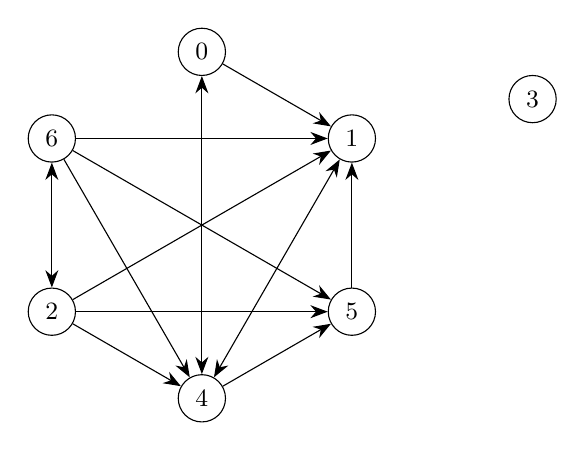
\begin{tikzpicture}[>={Stealth[length=2.2mm]},v/.style={circle,draw,inner sep=1.5pt,minimum size=6mm},font=\small]
\node[v] (v0) at (90:2.2) {$0$};
\node[v] (v1) at (30:2.2) {$1$};
\node[v] (v5) at (-30:2.2) {$5$};
\node[v] (v4) at (-90:2.2) {$4$};
\node[v] (v2) at (-150:2.2) {$2$};
\node[v] (v6) at (150:2.2) {$6$};
\node[v] (v3) at (4.2,1.6) {$3$};
\draw[->] (v0) -- (v1);
\draw[<->] (v0) -- (v4);
\draw[<->] (v1) -- (v4);
\draw[->] (v2) -- (v1);
\draw[->] (v2) -- (v4);
\draw[->] (v2) -- (v5);
\draw[<->] (v2) -- (v6);
\draw[->] (v4) -- (v5);
\draw[->] (v5) -- (v1);
\draw[->] (v6) -- (v1);
\draw[->] (v6) -- (v4);
\draw[->] (v6) -- (v5);
\end{tikzpicture}
\caption{The digraph $G_7$. Vertex $3$ sends an arc to every other vertex and receives arcs from $1$, $2$, $4$, $5$ and $6$; those arcs are not drawn. A double-headed line is a pair of opposite arcs.}\label{fig:G7}
\end{figure}

\begin{lemma}\label{lem:G7}
$G_7$ is strongly connected, satisfies (i) and (ii), and has no Hamilton cycle.
\end{lemma}

\begin{proof}
The in-neighborhoods are $N^-(0)=\{3,4\}$, $N^-(1)=\{0,2,3,4,5,6\}$, $N^-(2)=\{3,6\}$, $N^-(3)=\{1,2,4,5,6\}$, $N^-(4)=\{0,1,2,3,6\}$, $N^-(5)=\{2,3,4,6\}$ and $N^-(6)=\{2,3\}$. Both degree sequences are $(2,2,2,4,5,5,6)$. For $i=1$ the first alternatives of (i) and (ii) hold, since $d^+_1=d^-_1=2$. For $i=2,3$ the second alternatives hold, since $d^+_{7-i}=d^-_{7-i}=7-i$. Vertex $3$ sends an arc to every other vertex, and every other vertex reaches $3$ ($0\to1\to3$, and the others directly), so $G_7$ is strongly connected.

Suppose $f$ is the successor map of a Hamilton cycle. Since $N^-(2)=\{3,6\}$ and $N^-(6)=\{2,3\}$, and $2\to6\to2$ would close the cycle too early, either $f(3)=2$ and $f(2)=6$, or $f(3)=6$ and $f(6)=2$; in both cases $f(3)\in\{2,6\}$. Hence the predecessor of $0$, which lies in $N^-(0)=\{3,4\}$, is $4$, and $f(0)\in\{1,4\}\setminus\{4\}$ gives $f(0)=1$. Then $f(1)\in\{3,4\}$, and $f(1)=4$ would close the cycle $4\to0\to1\to4$ too early, so $f(1)=3$. The cycle is therefore $4\to0\to1\to3\to x\to y\to5\to4$ with $\{x,y\}=\{2,6\}$, which needs the arc $5\to4$. There is no such arc.
\end{proof}

\subsection{Six vertices}
Let $G_6$ have vertices $0,\dots,5$ and out-neighborhoods $N^+(0)=\{1,2,3,4,5\}$, $N^+(1)=\{4,5\}$, $N^+(2)=\{1,5\}$, $N^+(3)=\{1,4\}$, $N^+(4)=\{0,1,3,5\}$ and $N^+(5)=\{0,1,2,4\}$. It is isomorphic to Guninski's $g_2$~\cite{Gu20}.

\begin{lemma}\label{lem:G6}
$G_6$ is strongly connected, satisfies (i) and (ii), and has no cycle through both $2$ and $3$; in particular it has no Hamilton cycle.
\end{lemma}

\begin{proof}
Both degree sequences are $(2,2,2,4,4,5)$. For $i=1$ the first alternatives of (i) and (ii) hold, and for $i=2$ the second, since $d^+_4=d^-_4=4$. (Condition (iii) fails, since $d^+_3=d^-_3=2$.) Vertex $0$ sends an arc to every other vertex, and every vertex reaches $0$ ($4\to0$, $5\to0$, $1\to4$, $2\to5$, $3\to4$), so $G_6$ is strongly connected.

Suppose a cycle passes through $2$ and $3$, say $3\to P\to2\to Q\to3$ with paths $P$ and $Q$ that share no vertex. The predecessor of $2$ is $0$ or $5$, that of $3$ is $0$ or $4$, the successor of $2$ is $1$ or $5$, and that of $3$ is $1$ or $4$. If $P$ ends at $0$, then $Q$ ends at $4$, so $P$ starts at $1$; since $N^+(1)=\{4,5\}$, $P$ is $1\to5\to0$, and $2$ has no successor left. If $P$ ends at $5$, then $Q$ starts at $1$ and continues to $4$, since $N^+(1)=\{4,5\}$; so $Q$ is $1\to4$ or $1\to4\to0$, and $3$ has no successor left. Both cases are impossible.
\end{proof}

\subsection{A family for every \texorpdfstring{$n\ge8$}{n >= 8}}
For an integer $u\ge4$ let $F_u$ have $n=u+4$ vertices: a set $U$ of $u$ vertices with a distinguished vertex $w\in U$, and four further vertices $s$, $t$, $r_1$, $r_2$. Its arcs are
\begin{itemize}
\item $x\to y$ for every $x\in U$ and every vertex $y\ne x$;
\item $a\to b$ for all distinct $a,b\in L=\{t,r_1,r_2\}$;
\item $s\to t$, $s\to w$ and $t\to w$.
\end{itemize}
Figure~\ref{fig:F} shows the arcs that do not start in $U$.

\begin{figure}[ht]
\centering
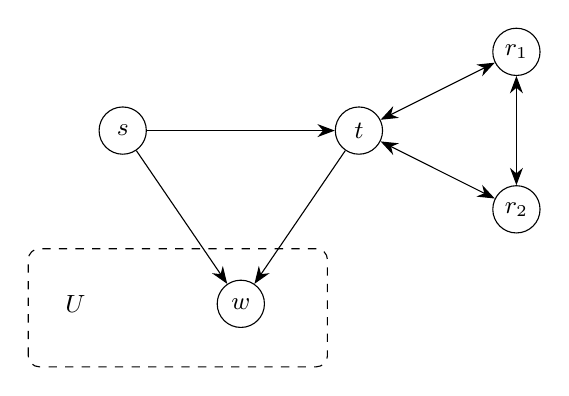
\begin{tikzpicture}[>={Stealth[length=2.2mm]},v/.style={circle,draw,inner sep=1.5pt,minimum size=6mm},font=\small]
\node[v] (s) at (0,0) {$s$};
\node[v] (t) at (3,0) {$t$};
\node[v] (r1) at (5,1) {$r_1$};
\node[v] (r2) at (5,-1) {$r_2$};
\node[v] (w) at (1.5,-2.2) {$w$};
\draw[rounded corners,dashed] (-1.2,-3) rectangle (2.6,-1.5);
\node at (-0.6,-2.2) {$U$};
\draw[->] (s) -- (t);
\draw[->] (s) -- (w);
\draw[->] (t) -- (w);
\draw[<->] (t) -- (r1);
\draw[<->] (t) -- (r2);
\draw[<->] (r1) -- (r2);
\end{tikzpicture}
\caption{The arcs of $F_u$ that do not start in $U$. Every vertex of $U$ also sends an arc to every other vertex.}\label{fig:F}
\end{figure}

\begin{lemma}\label{lem:F}
For every $u\ge4$, $F_u$ is strongly connected, satisfies (i), (ii) and, if $n=u+4$ is even, (iii), and has no Hamilton cycle. Moreover $s$ lies on no cycle with $r_1$, and none with $r_2$.
\end{lemma}

\begin{proof}
Out-degrees: $s$, $r_1$ and $r_2$ have out-degree $2$, $t$ has $3$, and every vertex of $U$ has $n-1$. In-degrees: each vertex of $U\setminus\{w\}$ receives arcs only from the other $u-1$ vertices of $U$; $s$ receives arcs from $U$ alone; $w$ receives arcs from $U\setminus\{w\}$, $s$ and $t$; $r_1$ and $r_2$ from $U$ and the other two vertices of $L$; and $t$ from every other vertex. So
\[
(d^+_1,\dots,d^+_n)=(2,2,2,3,n-1,\dots,n-1),\qquad
(d^-_1,\dots,d^-_n)=(n-5,\dots,n-5,\,n-4,\,n-3,\,n-2,\,n-2,\,n-1),
\]
with $u-1$ entries $n-5$, so that $d^-_{n-j}=n-j$ for $j=2,3,4$. Condition (i) holds for $i=1$ since $d^+_1=2$, for $i=2,3,4$ since $d^-_{n-i}=n-i$, and for $i\ge5$ since $d^+_i=n-1$. For condition (ii), every $i<n/2$ has $n-i>n/2\ge4$, so $d^+_{n-i}=n-1\ge n-i$. If $n$ is even, then $d^+_{n/2}=n-1$ when $n\ge10$, and $d^-_4=n-4=4$ when $n=8$; so (iii) holds. The vertex $w$ sends an arc to every other vertex, and every vertex reaches $w$ (vertices of $U$, $s$ and $t$ directly, $r_1$ and $r_2$ through $t$), so $F_u$ is strongly connected.

The only arc leaving $L$ is $t\to w$. Let $C$ be a cycle through $s$ that meets $L$. It must leave $L$, so it uses $t\to w$; it uses that arc only once, so it makes a single visit to $L$, which ends at $t$. Since $t$ precedes $w$ on $C$, the vertex $s$, whose out-neighbors are $t$ and $w$, precedes $t$. So the visit to $L$ also begins at $t$ and consists of $t$ alone. Hence no cycle passes through $s$ and $r_1$, or $s$ and $r_2$, and in particular no cycle passes through every vertex.
\end{proof}

\begin{proof}[Proof of Theorems~\ref{thm:main}(a) and~\ref{thm:pairs} and of Corollary~\ref{cor:NW}]
For $n=7$ take $G_7$ (Lemma~\ref{lem:G7}; condition (iii) is void for odd $n$), and for $n\ge8$ take $F_{n-4}$ (Lemma~\ref{lem:F}). These digraphs are strongly connected, so they are counterexamples to Conjecture~\ref{conj:NW} too; for $n=6$, Guninski's counterexamples, among them $G_6$ (Lemma~\ref{lem:G6}), refute it. The case $3\le n\le5$ of Corollary~\ref{cor:NW} is Theorem~\ref{thm:main}(b). Theorem~\ref{thm:pairs} is Lemma~\ref{lem:G6} for $n=6$ and Lemma~\ref{lem:F} for $n\ge8$.
\end{proof}

\section{Small orders}\label{sec:small}
Theorem~\ref{thm:main}(b) is proved by exhaustive search over all labeled digraphs on $3\le n\le6$ vertices: each of the $\binom n2$ pairs of vertices carries no arc, one of two arcs, or both, giving $4^{\binom n2}$ digraphs, or $2^{30}\approx1.07\times10^9$ for $n=6$. For each digraph the search tests (i), (ii) and (iii), strong connectivity and Hamiltonicity. Table~\ref{tab:small} lists the counts. A digraph is counted in the last column when it satisfies (i), (ii) and, for even $n$, (iii), and has no Hamilton cycle; it is counted in the fourth when it is strongly connected, satisfies (i) and (ii), and has no Hamilton cycle.

\begin{table}[ht]
\centering
\begin{tabular}{rrrrr}
$n$ & digraphs & satisfying (i), (ii) & counterexamples to Conj.~\ref{conj:NW} & counterexamples to Conj.~\ref{conj:KOT}\\\hline
3 & 64 & 7 & 0 & 0\\
4 & 4096 & 186 & 0 & 0\\
5 & 1048576 & 40140 & 0 & 0\\
6 & 1073741824 & 44387496 & 1080 & 0
\end{tabular}
\caption{Labeled digraphs on $n$ vertices. The 1080 labeled counterexamples to Conjecture~\ref{conj:NW} on six vertices all violate (iii).}\label{tab:small}
\end{table}

Two independent programs, which use different enumerations and different tests for the conditions, strong connectivity and Hamiltonicity (Appendix~\ref{app:programs}), produce identical output. The run at $n=6$ takes about 2.5 minutes on one core for the first and 1.5 minutes for the second.

\section{Verification and reproducibility}\label{sec:verification}

\paragraph{Formal verification.} The counterexamples are checked in Lean~4 with the Mathlib library~\cite{Lean,Mathlib}. A digraph on $n$ vertices is a Boolean relation on \texttt{Fin n} with no loops, so a pair of vertices may carry arcs in both directions:
\begin{verbatim}
structure Digraph (n : ℕ) where
  adj : Fin n → Fin n → Bool
  loopless : ∀ v, adj v v = false
\end{verbatim}
\texttt{G.dplus i} and \texttt{G.dminus i} are the $i$-th entries of the sorted out- and in-degree lists. The hypotheses read
\begin{verbatim}
def NWHyp (G : Digraph n) : Prop :=
  ∀ i, 1 ≤ i → 2 * i < n →
    (G.dplus i ≥ i + 1 ∨ G.dminus (n - i) ≥ n - i) ∧
    (G.dminus i ≥ i + 1 ∨ G.dplus (n - i) ≥ n - i)

def KOTHyp (G : Digraph n) : Prop :=
  NWHyp G ∧ (n % 2 = 0 → G.dplus (n / 2) ≥ n / 2 ∨ G.dminus (n / 2) ≥ n / 2)
\end{verbatim}
A Hamilton cycle (\texttt{HasHamCycle}) is a bijection $c$ of \texttt{Fin n} with an arc from $c(k)$ to $c(k+1 \bmod n)$ for every $k$; \texttt{StronglyConnected} is reflexive-transitive reachability for every ordered pair; and \texttt{CycleThrough G a b} asks for an injective map $c\colon\mathtt{Fin\ m}\to\mathtt{Fin\ n}$ with arcs from $c(k)$ to $c(k+1\bmod m)$ whose image contains $a$ and $b$. The digraph $F_u$ is \texttt{F u} on the vertices $0,\dots,u+3$, with $U=\{0,\dots,u-1\}$, $w=0$, $s=u$, $t=u+1$, $r_1=u+2$ and $r_2=u+3$. The main formal theorems are
\begin{verbatim}
theorem kot_counterexample_all (n : ℕ) (hn : 7 ≤ n) :
    ∃ G : Digraph n, KOTHyp G ∧ ¬ HasHamCycle G
theorem counterexample_all (n : ℕ) (hn : 6 ≤ n) :
    ∃ G : Digraph n, StronglyConnected G ∧ NWHyp G ∧ ¬ HasHamCycle G
theorem F_counterexample (u : ℕ) (hu : 4 ≤ u) :
    StronglyConnected (F u) ∧ NWHyp (F u) ∧ ¬ HasHamCycle (F u)
theorem F_no_cycle_through_s_r1 (u : ℕ) :
    ¬ CycleThrough (F u) ⟨u, _⟩ ⟨u + 2, _⟩
theorem G6_no_cycle_through_2_3 : ¬ CycleThrough G6 2 3
\end{verbatim}
together with \texttt{G6\_counterexample} and \texttt{G7\_counterexample} (strong connectivity, \texttt{NWHyp} and no Hamilton cycle), \texttt{F\_no\_cycle\_through\_s\_r2}, the lemma \texttt{F\_kot3} (condition (iii) for \texttt{F u} when $u\ge4$ and $u+4$ is even), and \texttt{not\_kotConjecture6} and \texttt{not\_nashWilliamsConjecture}, the negations of Conjectures~\ref{conj:KOT} and~\ref{conj:NW} stated for all $n\ge3$. Theorem~\ref{thm:main}(a) is \texttt{kot\_counterexample\_all}, whose witnesses are $G_7$ and \texttt{F (n-4)}, together with the strong connectivity in \texttt{G7\_counterexample} and \texttt{F\_counterexample}; no single formal statement combines the three properties. Corollary~\ref{cor:NW} for $n\ge6$ is \texttt{counterexample\_all}. Theorem~\ref{thm:pairs} combines \texttt{G6\_counterexample} and \texttt{G6\_no\_cycle\_through\_2\_3} for $n=6$, and \texttt{F\_counterexample}, \texttt{F\_kot3} and \texttt{F\_no\_cycle\_through\_s\_r1} for $n\ge8$; the pair statements hold for every $u$. The degree conditions for $F_u$ are proved for all $u\ge4$ through the counting form of Appendix~\ref{app:programs}, and the statements about $G_6$ and $G_7$ by decision procedures evaluated in Lean's kernel. The build checks the statements and that each theorem depends only on the axioms \texttt{propext}, \texttt{Classical.choice} and \texttt{Quot.sound}. Theorem~\ref{thm:main}(b) is not in Lean.

\paragraph{Computational checks.} Two further programs, written independently of each other and of the Lean development, read $G_6$ and $G_7$ from files and build $F_{n-4}$ for $8\le n\le18$ and $8\le n\le14$ respectively. They confirm strong connectivity, conditions (i)--(iii) and non-Hamiltonicity, and both reject four altered inputs: $G_6$ with the arc $2\to3$ added and $G_7$ with $0\to2$ added, which are Hamiltonian; $G_6$ without $4\to3$, which violates (ii); and $G_6$ with a loop. The two enumerators of Section~\ref{sec:small} complete the checks. The files, with the commands that run them, are published with this paper, in the folder \texttt{results/hamiltonian-degree-sequences} of its repository, together with the Lean development.

\begin{appendices}
\section{The programs}\label{app:programs}
Both the checkers and the enumerators come in two independent versions. The first enumerator assigns each pair of vertices one of its four states; it tests the conditions in their sorted-sequence form, strong connectivity by a reachability closure, and Hamiltonicity by the Held--Karp dynamic program over vertex subsets. The second runs through the $2^{n(n-1)}$ bit words over the ordered pairs of distinct vertices. It tests the conditions in their counting form, $d^+_i\ge i+1$ if and only if at most $i-1$ vertices have out-degree at most $i$, and $d^-_{n-i}\ge n-i$ if and only if at least $i+1$ vertices have in-degree at least $n-i$ (and likewise with out- and in-degrees exchanged); it tests strong connectivity by Warshall's transitive closure and Hamiltonicity by depth-first search over paths from a fixed vertex. The two checkers of Section~\ref{sec:verification} use the same pairs of methods: the first in Python with graph search in both directions for strong connectivity, the second in C.
\end{appendices}

\begin{thebibliography}{99}
\bibitem{AAY} J.~Adamus, L.~Adamus and A.~Yeo, On the Meyniel condition for hamiltonicity in bipartite digraphs, \emph{Discrete Math. Theor. Comput. Sci.} \textbf{16} (2014), no.~1. \href{https://doi.org/10.46298/dmtcs.1264}{doi:10.46298/dmtcs.1264}.
\bibitem{AM} D.~Amar and Y.~Manoussakis, Cycles and paths of many lengths in bipartite digraphs, \emph{J. Combin. Theory Ser. B} \textbf{50} (1990), 254--264. \href{https://doi.org/10.1016/0095-8956(90)90081-A}{doi:10.1016/0095-8956(90)90081-A}.
\bibitem{BT} J.-C.~Bermond and C.~Thomassen, Cycles in digraphs---a survey, \emph{J. Graph Theory} \textbf{5} (1981), 1--43. \href{https://doi.org/10.1002/jgt.3190050102}{doi:10.1002/jgt.3190050102}.
\bibitem{Ch} V.~Chvátal, On Hamilton's ideals, \emph{J. Combin. Theory Ser. B} \textbf{12} (1972), 163--168. \href{https://doi.org/10.1016/0095-8956(72)90020-2}{doi:10.1016/0095-8956(72)90020-2}.
\bibitem{CKKO} D.~Christofides, P.~Keevash, D.~Kühn and D.~Osthus, A semi-exact degree condition for Hamilton cycles in digraphs, \emph{SIAM J. Discrete Math.} \textbf{24} (2010), 709--756. \href{https://doi.org/10.1137/090761756}{doi:10.1137/090761756}; \href{https://arxiv.org/abs/1002.3910}{arXiv:1002.3910}.
\bibitem{Da} S.~Kh.~Darbinyan, On three conjectures of Thomassen and the extremal digraphs for two conjectures of Nash-Williams, \emph{J. Graph Theory} \textbf{109} (2025), 412--425. \href{https://doi.org/10.1002/jgt.23233}{doi:10.1002/jgt.23233}.
\bibitem{De} L.~DeBiasio, Inheritance of expansion and oriented Hamilton cycles in robust expanders: a regularity-free proof, preprint, October 2026. \href{https://arxiv.org/abs/2610.09072}{arXiv:2610.09072}.
\bibitem{Gu13} G.~Guninski, A counterexample to a conjecture of Nash-Williams about hamiltonicity of digraphs?, MathOverflow question 124217 (March 2013), with comments by G.~Royle, H.~Thomas and G.~C.~Drummond-Cole and an answer by L.~DeBiasio (August 2020). \url{https://mathoverflow.net/questions/124217}.
\bibitem{Gu20} G.~Guninski, Two more counterexamples to a conjecture from 1975 about hamiltonicity of digraphs, MathOverflow question 369168 (August 2020), with comments by L.~DeBiasio. \url{https://mathoverflow.net/questions/369168}.
\bibitem{Gu20b} G.~Guninski, Infinitely many counterexamples to Nash-Williams's conjecture about hamiltonicity?, MathOverflow question 369235 (August 2020). \url{https://mathoverflow.net/questions/369235}.
\bibitem{KO} D.~Kühn and D.~Osthus, A survey on Hamilton cycles in directed graphs, \emph{European J. Combin.} \textbf{33} (2012), 750--766. \href{https://doi.org/10.1016/j.ejc.2011.09.030}{doi:10.1016/j.ejc.2011.09.030}; \href{https://arxiv.org/abs/1006.0590v1}{arXiv:1006.0590v1}.
\bibitem{KOT} D.~Kühn, D.~Osthus and A.~Treglown, Hamiltonian degree sequences in digraphs, \emph{J. Combin. Theory Ser. B} \textbf{100} (2010), 367--380. \href{https://arxiv.org/abs/0807.1827v1}{arXiv:0807.1827v1} (July 2008) and \href{https://arxiv.org/abs/0807.1827v2}{v2} (December 2009).
\bibitem{Lean} L.~de~Moura and S.~Ullrich, The Lean 4 theorem prover and programming language, in \emph{Automated Deduction -- CADE 28}, Lecture Notes in Comput. Sci. \textbf{12699}, Springer, 2021, 625--635. \href{https://doi.org/10.1007/978-3-030-79876-5_37}{doi:10.1007/978-3-030-79876-5\_37}.
\bibitem{Mathlib} The mathlib Community, The Lean mathematical library, in \emph{Proceedings of the 9th ACM SIGPLAN International Conference on Certified Programs and Proofs}, 2020, 367--381. \href{https://doi.org/10.1145/3372885.3373824}{doi:10.1145/3372885.3373824}.
\bibitem{NW75} C.~St.~J.~A.~Nash-Williams, Hamiltonian circuits, in D.~R.~Fulkerson (ed.), \emph{Studies in Graph Theory, Part II}, MAA Studies in Mathematics \textbf{12}, Math. Assoc. Amer., Washington, D.C., 1975, 301--360.
\end{thebibliography}

\end{document}
